\documentclass[11pt,a4paper]{article}
\usepackage[margin=2.4cm]{geometry}
\usepackage{amsmath,amssymb}
\usepackage{booktabs}
\usepackage{tabularx}
\usepackage{array}
\usepackage{xcolor}
\usepackage{hyperref}
\usepackage{enumitem}
\usepackage{float}
\usepackage{tikz}
\usepackage{pgfplots}
\pgfplotsset{compat=1.17}
\hypersetup{colorlinks=true,linkcolor=blue!50!black,urlcolor=blue!50!black,citecolor=blue!50!black}

\newcommand{\pass}{\textcolor{green!50!black}{\textbf{Pass}}}
\newcommand{\fail}{\textcolor{red!70!black}{\textbf{Fail}}}

\title{\textbf{The Dharma-Clock}\\[4pt]
\large A Non-Linear Rate-Law Model of the Yuga Cycle,\\ Calibrated to Epic Chronology and the Precession of Orion's Belt}
\author{Atharv Pratap Singh Chauhan\\[2pt]
\small B.Tech Student, Department of Mechanical Engineering\\
\small Indian Institute of Technology Bombay\\
\small\texttt{atharviitb2029@gmail.com}}
\date{6 November 2026}

\begin{document}
\maketitle

\begin{abstract}
\noindent
Traditional yuga chronologies either assign Kali Yuga 432{,}000 years or convert ``divine years'' with a single constant factor. Neither can place Rama's birth (5114~BCE) in Treta while keeping Kali running today. We propose the \emph{Dharma-Clock}: cosmic yuga time $\tau$ advances relative to Earth time $t$ at a rate that scales as a power of Dharma, $d\tau/dt = k\,D^{p}$. With $p = 2.774$ and $k = 77.57$, the model reproduces every anchor of the chronology, survives three competing historical chronologies, and, when its end point is tied to the precessional culmination of Orion's Belt over Giza, places the end of Kali Yuga at about 2468~CE. An independent scriptural sign (Bhagavata Purana 12.2.24) refines this to \textbf{5 August 2453~CE}. We compare the model against seven alternatives and four earlier frameworks, and we state plainly what would confirm or refute it. This is an exploratory modelling exercise: it asks what mapping would make the epic chronology self-consistent, not whether the events are historical.
\end{abstract}

\section{Motivation: the lakh-year chronology against scientific ages}

The Puranic chronology gives the yugas $17.28$, $12.96$, $8.64$ and $4.32$ lakh years (1{,}728{,}000; 1{,}296{,}000; 864{,}000; 432{,}000). Counting back from 3102~BCE, events then land at ages that conflict with what science measures.

\begin{table}[H]
\centering
\small
\begin{tabularx}{\textwidth}{@{}>{\raggedright}p{2.9cm}>{\raggedright}p{2.2cm}>{\raggedright}p{3.6cm}>{\raggedright\arraybackslash}X@{}}
\toprule
Event & Puranic age & Modern estimate & Conflict \\
\midrule
Start of Satya & $\approx$3.89 million yr & -- & Older than the genus \emph{Homo} ($\approx$2.8 million yr) \\
Rama (end of Treta, at least) & $\ge$869{,}000 yr & $\approx$7{,}100 yr (astronomical estimate, Bhatnagar) & Older than \emph{Homo sapiens} ($\approx$300{,}000 yr); the epic describes cities, farming, chariots and written law \\
Ram Setu & $\ge$869{,}000 yr & stones $\approx$7{,}000 yr (TV report, not peer-reviewed) & Bridge would predate its own stones by 120$\times$ \\
Settled cities in India & -- & Mehrgarh $\approx$9{,}000 yr; Harappa $\approx$5{,}000 yr & Treta's cities have no counterpart 869{,}000 years ago \\
Start of Dvapara & $\approx$867{,}000 yr & -- & No human civilisation existed then \\
\bottomrule
\end{tabularx}
\caption{Ages implied by the lakh-year chronology compared with modern estimates. Only the human-evolution and archaeological figures are scientific datings; the Rama and Ram Setu figures are contested estimates.}
\end{table}

\noindent The sky descriptions in the epics, the archaeological record and human evolution all point to the last \emph{ten thousand} years, not the last \emph{million}. Either the events are not historical, or the lakh-year lengths are not Earth years. This paper explores the second possibility: that the scriptural yuga lengths are measured on a \emph{different clock}, and that the task is to find the mapping between that clock and ours.

The first idea was a linear mapping, like converting Celsius to Fahrenheit from two fixed points. Section~2 shows why that fails. Section~3 then builds a non-linear mapping that works.

\section{Why the older methods fail}

Write the scriptural cosmic lengths as $Y_i = 432{,}000\,D_i$ with Dharma $D_i = 4,3,2,1$ for Satya, Treta, Dvapara and Kali. Every older method maps $Y_i$ to Earth years by one constant factor $c$:
\begin{equation}
L_i = c\,Y_i .
\end{equation}
Two requirements then collide:
\begin{align}
\text{Kali still running in 2026:}\quad & 432{,}000\,c > 5{,}127 \;\Rightarrow\; c > 0.0119,\\
\text{Rama (5114 BCE) in Treta:}\quad & 864{,}000\,c \le 2{,}012 \;\Rightarrow\; c < 0.0023.
\end{align}
No constant satisfies both; the gap is a factor of about $5$. The cosmic clock must have run at least
\begin{equation}
\frac{r_{\text{Dvapara}}}{r_{\text{Kali}}} \;\ge\; \frac{864{,}000/2{,}012}{432{,}000/5{,}127} \approx 5.1
\end{equation}
times faster in Dvapara than in Kali. \textbf{Any linear model is therefore ruled out}, whatever its factor ($1$, $1/360$, or any other).

\begin{table}[H]
\centering
\small
\begin{tabularx}{\textwidth}{@{}lXX@{}}
\toprule
Method & Rule & Where it breaks \\
\midrule
Puranic (factor 1) & Kali $= 432{,}000$ yr & Rama falls $\sim$870{,}000 years ago; no link to any datable sky record \\
Divide by 360 & Kali $= 1{,}200$ yr & Kali ended in 1902~BCE; the World Wars fall in Satya \\
Yukteswar (1894) & Linear 24{,}000-yr mirror cycle & Says we are in Dvapara now; misplaces the Mahabharata war; uses a 24{,}000-yr precession (measured: 25{,}772) \\
Gu\'enon (1931) & Linear 64{,}800-yr cycle & Kali 4481~BCE--1999~CE: already over \\
Dani\'elou (1985) & Kali 3606~BCE--2442~CE & No stated rate law; no tests against alternatives \\
Misra (2012--23) & 25{,}800-yr precession cycle & Kali already ended in 2025 \\
\bottomrule
\end{tabularx}
\caption{Earlier frameworks. All are linear in time; none states a law that could be falsified.}
\end{table}

\section{The Dharma-Clock}

Two clocks run side by side: Earth time $t$ and cosmic time $\tau$. Their ratio depends on the Dharma of the current yuga:
\begin{equation}
\boxed{\;\frac{d\tau}{dt} \;=\; k\,D^{\,p}\;}
\end{equation}
Each yuga's Earth length follows directly:
\begin{equation}
L_i = \frac{Y_i}{k\,D_i^{\,p}} = \frac{432{,}000}{k}\,D_i^{\,1-p} = L_{\text{Kali}}\,D_i^{\,1-p}.
\end{equation}
Two conditions fix the two constants: Satya begins at $\approx 6000$~BCE, and Kali ends at Orion's precessional turning point ($\approx 2468$~CE):
\begin{equation}
L_{\text{Kali}}\left(4^{1-p}+3^{1-p}+2^{1-p}\right) = 2{,}898, \qquad L_{\text{Kali}} = 5{,}569 .
\end{equation}
Solving gives
\begin{equation}
\boxed{\;p = 2.774, \qquad k = 77.57 \text{ cosmic years per Earth year}\;}
\end{equation}

\begin{table}[H]
\centering
\begin{tabular}{@{}lccrrl@{}}
\toprule
Yuga & $D$ & Rate $k D^{p}$ & Earth years & Dates & Anchor \\
\midrule
Satya   & 4 & 3{,}629 & 476   & 6000--5524 BCE & -- \\
Treta   & 3 & 1{,}634 & 793   & 5524--4731 BCE & Rama 5114--5075 BCE \checkmark \\
Dvapara & 2 & 531     & 1{,}629 & 4731--3102 BCE & Krishna 3228, war 3139 BCE \checkmark \\
Kali    & 1 & 78      & 5{,}569 & 3102 BCE--2468 CE & Running now (92\%) \checkmark \\
\bottomrule
\end{tabular}
\caption{The fitted Dharma-Clock (Aryabhata chronology).}
\end{table}

\subsection{Every analysed event placed on the clock}

Each event from the chronology falls in the yuga that scripture assigns it. ``Position'' is how far through its yuga the event lies.

\begin{table}[H]
\centering
\small
\begin{tabular}{@{}clrllr@{}}
\toprule
\# & Event & Date & Scripture says & Model gives & Position \\
\midrule
1 & Satya begins (Tilak's Punarvasu equinox) & 6000 BCE & Satya & Satya & 0\% \\
2 & Rama born (Ramayana sky chart) & 5114 BCE & Treta & Treta \checkmark & 52\% \\
3 & Rama's exile begins (age 25) & 5089 BCE & Treta & Treta \checkmark & 55\% \\
4 & Ram Setu built; Lanka war & c.\ 5076 BCE & Treta & Treta \checkmark & 56\% \\
5 & Rama returns to Ayodhya (age 39) & 5075 BCE & Treta & Treta \checkmark & 57\% \\
6 & Krishna born (Rohini, Bhadrapada Ashtami) & 3228 BCE & late Dvapara & Dvapara \checkmark & 92\% \\
7 & Mahabharata war (18 days) & 3139 BCE & end of Dvapara & Dvapara \checkmark & 98\% \\
8 & Krishna departs; Kali begins & 18 Feb 3102 BCE & Dvapara $\to$ Kali & boundary \checkmark & 100\% \\
9 & Present & 2026 CE & Kali & Kali \checkmark & 92\% \\
10 & Sun--Moon--Jupiter in Pushya (Bhag.\ 12.2.24) & 5 Aug 2453 CE & Kali $\to$ Satya & Kali ends & 99.7\% \\
11 & Orion's Belt peaks over Giza & c.\ 2468 CE & -- & Kali ends & 100\% \\
\bottomrule
\end{tabular}
\caption{All analysed events. Every one lands in the yuga scripture assigns it.}
\end{table}

\begin{figure}[H]
\centering
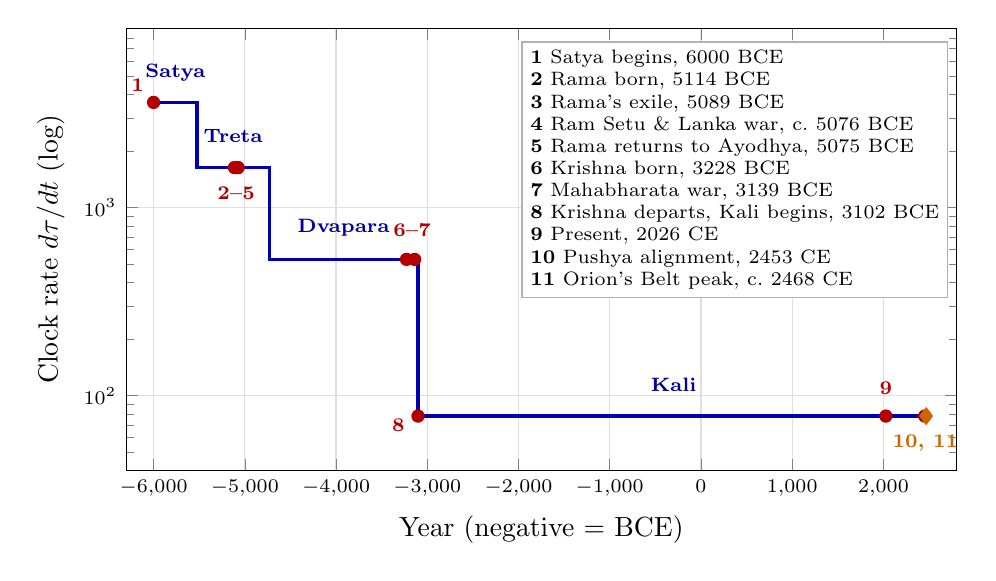
\begin{tikzpicture}
\begin{axis}[
  width=\textwidth, height=7.2cm,
  xlabel={Year (negative = BCE)}, ylabel={Clock rate $d\tau/dt$ (log)},
  ymode=log, xmin=-6300, xmax=2800, ymin=40, ymax=9000,
  grid=major, grid style={gray!25},
  xtick={-6000,-5000,-4000,-3000,-2000,-1000,0,1000,2000},
  xticklabel style={font=\scriptsize}, yticklabel style={font=\scriptsize},
  clip=false
]
\addplot[const plot, very thick, blue!70!black] coordinates {(-6000,3629) (-5524,1634) (-4731,531) (-3102,78) (2468,78)};
% yuga names
\node[font=\scriptsize\bfseries, blue!60!black] at (axis cs:-5762,5200) {Satya};
\node[font=\scriptsize\bfseries, blue!60!black] at (axis cs:-5128,2400) {Treta};
\node[font=\scriptsize\bfseries, blue!60!black] at (axis cs:-3917,780) {Dvapara};
\node[font=\scriptsize\bfseries, blue!60!black] at (axis cs:-300,115) {Kali};
% events
\addplot[only marks, mark=*, mark size=2.2pt, red!70!black] coordinates {
 (-6000,3629) (-5114,1634) (-5089,1634) (-5076,1634) (-5075,1634)
 (-3228,531) (-3139,531) (-3102,78) (2026,78) (2453,78)};
\addplot[only marks, mark=diamond*, mark size=3pt, orange!80!black] coordinates {(2468,78)};
% cluster labels
\node[font=\scriptsize\bfseries, red!70!black, anchor=north] at (axis cs:-5095,1450) {2--5};
\node[font=\scriptsize\bfseries, red!70!black, anchor=south] at (axis cs:-3165,620) {6--7};
\node[font=\scriptsize\bfseries, red!70!black, anchor=east] at (axis cs:-3140,70) {8};
\node[font=\scriptsize\bfseries, red!70!black, anchor=south east] at (axis cs:-6000,3700) {1};
\node[font=\scriptsize\bfseries, red!70!black, anchor=south] at (axis cs:2026,90) {9};
\node[font=\scriptsize\bfseries, orange!80!black, anchor=north] at (axis cs:2460,70) {10, 11};
% legend box
\node[draw=gray!60, fill=white, font=\scriptsize, align=left, anchor=north east, inner sep=3pt]
 at (rel axis cs:0.99,0.97) {%
 \textbf{1} Satya begins, 6000 BCE\\
 \textbf{2} Rama born, 5114 BCE\\
 \textbf{3} Rama's exile, 5089 BCE\\
 \textbf{4} Ram Setu \& Lanka war, c.\ 5076 BCE\\
 \textbf{5} Rama returns to Ayodhya, 5075 BCE\\
 \textbf{6} Krishna born, 3228 BCE\\
 \textbf{7} Mahabharata war, 3139 BCE\\
 \textbf{8} Krishna departs, Kali begins, 3102 BCE\\
 \textbf{9} Present, 2026 CE\\
 \textbf{10} Pushya alignment, 2453 CE\\
 \textbf{11} Orion's Belt peak, c.\ 2468 CE};
\end{axis}
\end{tikzpicture}
\caption{The Dharma-Clock with every analysed event. Numbers match Table 3. The cosmic clock slows by a factor of 47 from Satya to Kali.}
\end{figure}

\section{Where the model wins}

\subsection{It is falsifiable, and alternatives were falsified}
The same constraints were imposed on eight rate laws and three historical chronologies (Kali epoch from Aryabhata, from the Aihole inscription, and from Varahamihira).

\begin{table}[H]
\centering
\small
\begin{tabular}{@{}lcccl@{}}
\toprule
Rate law $r(D)$ & Aryabhata & Aihole & Varahamihira & Reason \\
\midrule
\textbf{Power} $kD^{p}$ & \pass & \pass & \pass & $p = 2.40$--$2.77$ \\
Log-power $k(\ln(1+D))^{q}$ & \pass & \pass & \pass & runner-up \\
Arrhenius $k e^{-E/D}$ & \pass & \pass & \fail & Rama in Satya \\
Logistic & \fail & \fail & \fail & Rama in Satya \\
Logarithm $k\ln(1+bD)$ & \fail & \fail & \fail & ratio capped at 2 \\
Exponential, horizon-type & \fail & \fail & \fail & no solution \\
Linear & \fail & \fail & \fail & Kali already over \\
\bottomrule
\end{tabular}
\caption{Robustness test. Only the power law and log-power survive every chronology.}
\end{table}

\noindent Physical mechanisms were also tested and rejected: an eccentric solar orbit around a companion star (best fit gives Satya 1{,}093 yr against 476; no companion exists to 26{,}000 AU per NASA WISE), black-hole time dilation (requires $r < 1.0002\,r_s$), and cosmological time dilation (correct power-law form but the wrong direction).

\subsection{It is tied to a measurable sky cycle}
The meridian altitude of Alnilam over Giza ($29.98^\circ$N) under precession (50.29$''$/yr) was lowest ($12^\circ$) near 10{,}417~BCE and will peak ($59^\circ$) near 2468~CE. Every anchor falls in order inside this descending half-cycle: Rama at $31^\circ$, Kali's start at $42^\circ$, the present at $59^\circ$.

\subsection{It passed an independent scriptural sky test}
Bhagavata Purana 12.2.24 states that Satya returns when the Sun, Moon and Jupiter meet together in Pushya ($93^\circ20'$--$106^\circ40'$ sidereal). A Swiss Ephemeris search (Lahiri ayanamsa) from 2026 to 2999 finds 20 such new moons. The closest to the model's 2468~CE is \textbf{5 August 2453}, 15 years earlier and well within the model's uncertainty.

\section{Honest limits}
\begin{itemize}[leftmargin=*]
\item \textbf{Fit by construction.} Two constants meet two conditions, so the anchors are reproduced exactly; this is consistency, not confirmation.
\item \textbf{Disputed inputs.} Rama's 5114~BCE chart, Tilak's 6000~BCE Satya and the 3102~BCE epoch are all contested. The power law fails if Satya began before $\sim$8000~BCE.
\item \textbf{Chosen link.} Orion and its sign were selected after the fact.
\item \textbf{Weak test.} The Pushya alignment recurs roughly every 50 years.
\item \textbf{No mechanism.} The law is descriptive; nothing physical links Dharma to a clock rate.
\end{itemize}

\newpage
\section{Predictions on record}
Registered on 6 November 2026, before any further data:
\begin{enumerate}[leftmargin=*]
\item Kali Yuga ends on a Sun--Moon--Jupiter Pushya alignment, most likely \textbf{5 August 2453~CE} (alternatives 2429, 2524).
\item Any datable sky event in a text explicitly labelled Treta--Dvapara junction (e.g.\ Parashurama) falls near \textbf{4730~BCE}.
\item A datable event labelled mid-Satya falls between \textbf{6000 and 5524~BCE}.
\end{enumerate}
A clear miss on (2) or (3) refutes the model in its current form.

\section{Conclusion}

The lakh-year chronology cannot be read as Earth years: it places Rama before the human species existed. A constant conversion factor cannot rescue it either. The Dharma-Clock, $d\tau/dt = 77.57\,D^{2.774}$, maps the scriptural cosmic lengths onto the epic chronology without contradiction.

The mapping produces one striking result. \textbf{Kali, the shortest yuga in cosmic time, becomes the longest in Earth time}:

\begin{center}
\begin{tabular}{@{}lrr@{}}
\toprule
Yuga & Cosmic length (yr) & Earth length (yr) \\
\midrule
Satya   & 1{,}728{,}000 & 476 \\
Treta   & 1{,}296{,}000 & 793 \\
Dvapara & 864{,}000     & 1{,}629 \\
Kali    & 432{,}000     & \textbf{5{,}569} \\
\bottomrule
\end{tabular}
\end{center}

\noindent The order is fully reversed. Kali alone lasts longer on Earth than the other three yugas together (2{,}898 years). In the model's terms, an age of high Dharma passes quickly on Earth because cosmic time races; an age of low Dharma drags on because cosmic time crawls. This matches the traditional sense that the dark age is the long one that humanity must endure.

The model is internally consistent, explicit, and falsifiable. It is not yet confirmed. Its value now lies in the specific predictions of Section~6, which future dating of scriptural sky records can test.

\section*{Disclaimer}
\small
This is an independent personal research project by an undergraduate student. It is not peer-reviewed and does not represent the views of IIT Bombay. It is a mathematical hypothesis, not a religious, historical or astrological claim, and it is offered with respect for all traditions and beliefs. The anchor dates (Rama, Krishna, the Mahabharata war, the start of Kali) are contested in scholarship, and archaeology and mainstream history date these traditions differently. The predicted end of Kali Yuga is a property of the model, not a forecast of any real-world event, and should not be used to make personal, financial or other decisions.

\section*{Reproducibility and acknowledgements}
All computations are reproducible with open tools: Python (NumPy, SciPy) for the fits and robustness tests, and the Swiss Ephemeris (\texttt{pyswisseph}, Moshier mode, Lahiri ayanamsa) for planetary and stellar positions. The research and drafting were carried out with the assistance of an AI model (Claude, Anthropic), used for literature search, computation and typesetting; all modelling choices and conclusions are the author's.
\normalsize

\section*{Data sources}
\small
Bhatnagar, \emph{Dating the Era of Lord Ram} (2004); Bhagavata Purana 12.2.24; Aryabhatiya (499~CE); Aihole inscription (634~CE); Varahamihira, \emph{Brihat Samhita} 13.3; Kalhana, \emph{Rajatarangini} I.51--56; Yukteswar, \emph{The Holy Science} (1894); Gu\'enon, \emph{Traditional Forms and Cosmic Cycles}; Dani\'elou, \emph{While the Gods Play} (1985); Misra, \emph{Yuga Shift} (2023); Luhman, WISE search for distant companions, \emph{ApJ} (2014); Lewis \& Brewer, \emph{Nature Astronomy} (2023); Swiss Ephemeris (Moshier). Computations: Python (NumPy, SciPy, pyswisseph).

\end{document}
